\documentclass[tikz, border=10pt]{standalone}
\usepackage{tikz}

\begin{document}
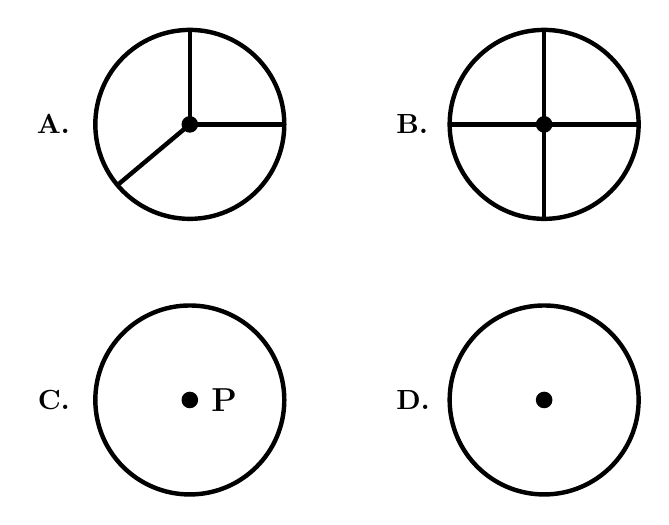
\begin{tikzpicture}

% Define radius
\def\r{1.2}

% ===== Top Left Circle (A) =====
\begin{scope}[shift={(0, 0)}]
    % Draw circle
    \draw[ultra thick] (0,0) circle (\r);
    
    % Draw center point
    \fill (0,0) circle (3pt);
    
    % Draw line going up-left (around 0 degrees)
    \draw[ultra thick] (0,0) -- (0:\r);
    
    % Draw line going down (90 degrees)
    \draw[ultra thick] (0,0) -- (90:\r);
    
    % Draw line going down (90 degrees)
    \draw[ultra thick] (0,0) -- (220:\r);
    
    % Label
    \node[left] at (-\r-0.2, 0) {\textbf{A.}};
\end{scope}

% ===== Top Right Circle (B) =====
\begin{scope}[shift={(4.5, 0)}]
    % Draw circle
    \draw[ultra thick] (0,0) circle (\r);
    
    % Draw center point
    \fill (0,0) circle (3pt);
    
    % Draw vertical line (top to bottom)
    \draw[ultra thick] (0,\r) -- (0,-\r);
    
    % Draw horizontal line (left to right)
    \draw[ultra thick] (-\r,0) -- (\r,0);
    
    % Label
    \node[right] at (-\r-0.8, 0) {\textbf{B.}};
\end{scope}

% ===== Bottom Left Circle (C) =====
\begin{scope}[shift={(0, -3.5)}]
    % Draw circle
    \draw[ultra thick] (0,0) circle (\r);
    
    % Draw center point
    \fill (0,0) circle (3pt);
    
    % Label P next to center point
    \node[right] at (0.15, 0) {\large\textbf{P}};
    
    % Label
    \node[left] at (-\r-0.2, 0) {\textbf{C.}};
\end{scope}

% ===== Bottom Right Circle (D) =====
\begin{scope}[shift={(4.5, -3.5)}]
    % Draw circle
    \draw[ultra thick] (0,0) circle (\r);
    
    % Draw center point
    \fill (0,0) circle (3pt);
    
    % Label
    \node[right] at (-\r-0.8, 0) {\textbf{D.}};
\end{scope}

\end{tikzpicture}
\end{document}